\documentclass[titlepage,a4paper]{article}
\usepackage[T1]{fontenc}		% font encode
\usepackage[utf8]{inputenc}	 % input encode
\usepackage[english]{babel}		% secondary and main languages
\usepackage{authblk}			% to add affiliation
\usepackage[tt]{titlepic}		% to add the logo in first page
\usepackage{graphicx}			% to add images
\usepackage{gensymb}			% used for symbols as °(\degree)
\usepackage{amsmath}
\usepackage{mathtools}			% used for math formulae
\usepackage{float}
\usepackage{titlesec}			%used to add \sectionbreak command
\usepackage{appendix}
\usepackage{hyperref}
\usepackage{footnote}
\usepackage{enumitem}
\usepackage{blindtext}
\usepackage{graphicx}
\usepackage{caption}
\usepackage{subcaption}
\usepackage{listings}
\usepackage{xcolor}
\usepackage{hyperref}
\usepackage{rotating}
\usepackage{siunitx}
\usepackage{listings}		%code listings (lstlisting)
\usepackage{color}

\setlistdepth{9}									% enumerate depth 
\newlist{req_enum}{enumerate}{9}					% definition of a new enumerate type
\setlist[req_enum]{label=\thesubsection.\arabic{*}.}	% include the chapter number

\definecolor{gray}{rgb}{0.4,0.4,0.4}
\definecolor{darkblue}{rgb}{0.0,0.0,0.6}
\definecolor{cyan}{rgb}{0.0,0.6,0.6}

\lstset{basicstyle=\ttfamily,columns=fullflexible,showstringspaces=false,tabsize=2}

\lstdefinestyle{custompython}{backgroundcolor=\color{white},belowcaptionskip=1\baselineskip,breaklines=true,frame=L,xleftmargin=\parindent,language=Python,showstringspaces=false,basicstyle=\footnotesize\ttfamily,keywordstyle=\bfseries\color{darkblue},commentstyle=\itshape\color{green!40!black},identifierstyle=\color{blue},stringstyle=\color{orange},
}


\lstdefinestyle{custombash}{basicstyle=\color{white},backgroundcolor=\color{black},belowcaptionskip=1\baselineskip,breaklines=true,frame=L,xleftmargin=\parindent,language=bash,showstringspaces=false,morekeywords={roslaunch,rosrun},basicstyle=\footnotesize\ttfamily,keywordstyle=\bfseries\color{yellow},commentstyle=\itshape\color{green},identifierstyle=\color{white},stringstyle=\color{orange},
}


\lstdefinelanguage{XML}{morestring=[b]", morestring=[s]{>}{<}, stringstyle=\color{red}, identifierstyle=\color{darkblue}, commentstyle=\color{green}, keywordstyle=\color{cyan}, morekeywords={name,xmlns,version,type}% list your attributes here
}

\newcommand{\sectionbreak}{\clearpage}	%to start new section in a new page

\graphicspath{{img/}{img/Johnny/}{img/rob/screenshots/}}

\renewcommand\Authfont{\fontsize{12}{14.4}\selectfont}
\renewcommand\Affilfont{\fontsize{10}{10.8}\selectfont}

%intestazione
\title{
\includegraphics[width=4cm, keepaspectratio]{unipi_blu}\hspace{2cm}
\includegraphics [width=4cm, keepaspectratio]{santanna}~\\[2cm]
\textbf{\LARGE Design of Embedded Systems}\\[1cm] ESSTA, Energy Saving Smart-home distributed Temperature control Application, Requirements}

\author{\emph{Falzone Giovanni}}
\affil{\emph{jointly M.Sc Embedded Computing Systems}}
\affil{\emph{Sant'Anna School of Advanced Studies}}
\affil{\emph{University of Pisa}}

\begin{document}
\maketitle
\tableofcontents

\section{Introduction}
The purpose of this project is to realize a smart-home application to control the heating system of a building based on the temperature of each room, in order to minimize the consumption of the building each room apply an energy saving function reducing the desired temperature when it is not needed.
The system is composed by two differ modules
\begin{itemize}
	\item central unit module 
	\item room module
\end{itemize}

\subsection{Central Unit}
The \textit{Central Unit} has the role of coordinator that retrieve the status of each room and computes the average values for the building.\\

\subsubsection{Graphical user interface}
Using a graphical User Interface the module represents the average values of the building and the values for each room, the graphical User Interface is composed by:
\begin{itemize}
	\item \textit{Main page} to represent the overview of the building
	\item \textit{Room page} to represent the status of each room
	\item \textit{Settings page} to set the desired temperature
\end{itemize}

Whenever the \textit{Main page} is selected the module shall represent the average values among all the rooms for \textit{Temperature}, \textit{Humidity} and \textit{Usage}.\\
Whenever the \textit{Main page} is selected the module shall represent the \textit{Energy Saving} if at least one room is set to \textbf{Energy Saving mode}.\\
Whenever the \textit{Main page} is selected the module shall represent the \textit{Warning} if at least one room is set to \textbf{crashed}.\\
Whenever the \textit{Main page} is selected the module shall allow the user to move in the \textit{Settings page}, next and previous \textit{Room page}.\\

Whenever the \textit{Settings page} is selected the module shall represent the \textit{Desired Temperature} and shall allow the user to increase or deacrease it by a factor of 0.5 C\degree in the range of 15 C\degree and 30 C\degree.\\
Whenever the \textit{Settings page} is selected the module shall represent the average values among all the rooms for \textit{Humidity} and \textit{Usage}.\\
Whenever the \textit{Settings page} is selected the module shall represent the \textit{Energy Saving} if at least one room is set to \textbf{Energy Saving mode}.\\
Whenever the \textit{Settings page} is selected the module shall represent the \textit{Warning} if at least one room is set to \textbf{crashed}.\\
Whenever the \textit{Settings page} is selected the module shall allow the user to move in the \textit{Main page}.\\

Whenever the \textit{Room page} is selected the module shall represent the average values among all the rooms for \textit{Temperature}, \textit{Humidity} and \textit{Usage}.\\
Whenever the \textit{Room page} is selected the module shall represent the \textit{Energy Saving} if at least one room is set to \textit{Energy Saving mode}.\\
Whenever the \textit{Room page} is selected the module shall represent the \textit{Warning} if at least one room is set to \textbf{crashed}.\\
Whenever the \textit{Room page} is selected the module shall allow the user to move in the \textit{Main page}, \textit{Settings page}, next and previous \textit{Room page}.\\

The graphical user interface shall represent the following information as reported in the table \ref{tab:GraphicalInformations}.
\begin{table}[H]
	\centering
			\begin{tabular}{||l | l||} 
			\hline
			\textbf{Information}	& \textbf{Format} \\ 
			\hline
			Temperature	& C\degree \\ 
			\hline
			Humidity	& \% \\ 
			\hline
			Usage		& \% \\ 
			\hline
			Energy Saving	& boolean \\ 
			\hline
			Warning		& boolean \\ 
			\hline
		\end{tabular}
		\captionof{table}{Display Information\label{tab:GraphicalInformations}}
\end{table}

\subsubsection{Communication}
Whenever a \textit{Room Request message} is sent and the \textit{Room Status message} is not received within 20s the module shall mark the room as \textbf{crashed}.
The module shall send the \textit{Room Request message} for each room at least every 30s.

%--------------------------------------
\subsection{Room Module}
The purpose of this module is to control the temperature of the room acting on a valve in order to 
reach and maintain the \textit{GoalTemperature}.

\subsubsection{Energy Saving mode}
In order to minimize the consumption the module keep tracks of the presence of motion inside the room
using a motion sensor. \\

If a motion is detected in the last 30s, the module shall set the \textit{GoalTemperature} to the one set by the user,otherwise the module shall set the \textit{GoalTemperature} to:

\begin{equation}
	GoalTemperature = DesiredTemperature - EnergySavingTemperatureOffset
\end{equation}
Whenever the module is in \textit{Energy Saving mode} it shall notify it through the \textit{Interface}.

\subsubsection{Valve control}
In order to control the heating of the room the valve is moved to different positions based on the temperature error 
(\textit{ActualTemperature} - \textit{GoalThemperature}) as in the following table, 
whenever one of these rules is valid the module shall move the valve in the correspondent position described in the third column of the table \ref{tab:ValvePositions} as percentage of maximum flow.
\begin{center}
	\begin{tabular}{| l | l | l |} 
		\hline
		\textbf{rule} & \textbf{valve position} & \textbf{Flow in \%}\\
		\hline
		\begin{math} error < -HIGH \end{math} &  OPEN\_POSITION & 100\\
		\hline
		\begin{math} error \in [-HIGH, -APPROCHING) \end{math}  & HIGH\_POSITION & 75\\
		\hline
		\begin{math} error \in [-APPROCHING, +APPROCHING] \end{math} & MIDDLE\_POSITION & 50 \\
		\hline
		\begin{math} error \in (APPROCHING, HIGH] \end{math} & LOW\_POSITION & 25\\
		\hline
		error > HIGH &  CLOSED\_POSITION & 0 \\
		\hline
	\end{tabular}
	\captionof{table}{\label{tab:ValvePositions}}
\end{center}
Whenever the valve is in \textit{OPEN\_POSITION} or \textit{CLOSED\_POSITION} the module shall check the position and set \textbf{Valve Error} if it is not valid.

In the following table\ref{tab:TemperatureThresholds} are reported the temperature thresholds:
\begin{center}
	\begin{tabular}{||l | l||} 
		\hline
		HIGH 		& 2 C\degree \\ 
		\hline
		APPROCHING 	& 1 C\degree \\ 
		\hline
	\end{tabular}
	\captionof{table}{\label{tab:TemperatureThresholds}}
\end{center}


\subsubsection{Communication}
Whenever a \textit{Room Request message} is not received within 60s the module shall send the \textit{Room Status Message} and set the \textbf{Communication error}.

\subsubsection{Errors}
Whenever one of the errors are set, the module shall notify it through the \textit{Interface}.
In the following table \ref{tab:RoomErrors} are reported the possible errors.
\begin{center}
	\begin{tabular}{|| l ||} 
		\hline
		\textbf{Valve error} \\ 
		\hline
		\textbf{Communication error} \\ 
		\hline
		\textbf{Sensor error} \\ 
		\hline
	\end{tabular}
	\captionof{table}{\label{tab:RoomErrors}}
\end{center}

\section{User Requirements}
	\subsection{Central Unit}
		\begin{req_enum}
			\item \textbf{Graphical User Interface on Central Unit module}
			\begin{req_enum}[label*=\arabic*.]
				\item \textbf{Main Page}
					\begin{req_enum}[label*=\arabic*.]
						\item Whenever the \textit{Main page} is selected the module shall represent the average values among all the rooms for \textit{Temperature}, \textit{Humidity} and \textit{Usage}.\\
						\item Whenever the \textit{Main page} is selected the module shall represent the \textit{Energy Saving} if at least one room is set to \textbf{Energy Saving mode}.\\
						\item Whenever the \textit{Main page} is selected the module shall represent the \textit{Warning} if at least one room is set to \textbf{crashed}.\\
						\item Whenever the \textit{Main page} is selected the module shall allow the user to move in the \textit{Settings page}, next and previous \textit{Room page}.\\
					\end{req_enum}
				\item \textbf{Settings Page}
					\begin{req_enum}[label*=\arabic*.]
						\item Whenever the \textit{Settings page} is selected the module shall represent the \textit{Desired Temperature} and shall allow the user to increase or deacrease it by a factor of 0.5 C\degree in the range of 15 C\degree and 30 C\degree.\\
						\item Whenever the \textit{Settings page} is selected the module shall represent the average values among all the rooms for \textit{Humidity} and \textit{Usage}.\\
						\item Whenever the \textit{Settings page} is selected the module shall represent the \textit{Energy Saving} if at least one room is set to \textbf{Energy Saving mode}.\\
						\item Whenever the \textit{Settings page} is selected the module shall represent the \textit{Warning} if at least one room is set to \textbf{crashed}.\\
						\item Whenever the \textit{Settings page} is selected the module shall allow the user to move in the \textit{Main page}.\\
					\end{req_enum}

				\item \textbf{Room Page}
					\begin{req_enum}[label*=\arabic*.]
						\item Whenever the \textit{Room page} is selected the module shall represent the average values among all the rooms for \textit{Temperature}, \textit{Humidity} and \textit{Usage}.\\
						\item Whenever the \textit{Room page} is selected the module shall represent the \textit{Energy Saving} if at least one room is set to \textbf{Energy Saving mode}.\\
						\item Whenever the \textit{Room page} is selected the module shall represent the \textit{Warning} if at least one room is set to \textbf{crashed}.\\
						\item Whenever the \textit{Room page} is selected the module shall allow the user to move in the \textit{Main page}, \textit{Settings page}, next and previous \textit{Room page}.\\
					\end{req_enum}
			\end{req_enum}
		\end{req_enum}

%------------------------------------------------------------------

	\subsection{Room}
		\begin{req_enum}
			\item \textbf{Energy Saving mode}
			\begin{req_enum}[label*=\arabic*.]
				\item Whenever a motion is detected in the last 30s the module shall move in \textbf{Enery Saving} mode and show it through the ENERGY\_SAVING\_LED
				\item Whenever a motion is detected shall show it through the ENERGY\_SAVING\_LED
			\end{req_enum}
		\end{req_enum}
\section{Functional requirements}
	\subsection{Central Unit}
		\begin{req_enum}
			\item \textbf{Communication}
				\begin{req_enum}[label*=\arabic*.]
					\item The \textit{Central Unit} shall send a \textit{Room Request message} polling among all the rooms
					\item The \textit{Room Request message} shall include the Id of the room and the \textit{Desired Temperature} in Celsius\degree
					\item The \textit{Room Status message} shall include the Id of the room, the \textit{Energy Saving mode} one if active zero otherwise, the \textit{Temperature} in Celsius\degree, the \textit{Humidity} in \% and the \textit{Valve position} in \%
					\item Whenever a \textit{Room Status message} is corrupted or doesn't arrive within 5s from the sent of the \textit{Room Request message}, the same \textit{Room Request message} shall be resent until 3 times before marking the room as \textbf{crashed}
				\end{req_enum}
		\end{req_enum}

%------------------------------------------------------------------

	\subsection{Room}
		\begin{req_enum}
			\item \textbf{Initialization}
				\begin{req_enum}[label*=\arabic*.]
					\item The module shall check the position of the valve moving in CLOSED, LOW, MIDDLE, HIGH and OPEN
					\item The module shall check the correctness of the sensors
					\item The module shall turn on all the LEDS and the turn off
				\end{req_enum}
			\item \textbf{Running}
			\begin{req_enum}[label*=\arabic*.]
				\item \textbf{Energy Saving mode}
					\begin{req_enum}[label*=\arabic*.]
						\item Whenever the module is in energy saving mode the module shall turn on the ENERGY\_SAVING\_LED
						\item Whenever the module is in energy saving mode the \textit{Goal Temperature} shall be set to the \textit{Desired Temperature} minus the \textit{Energy Saving Temperature Offset}
					\end{req_enum}

				\item \textbf{Normal mode}
					\begin{req_enum}[label*=\arabic*.]
						\item Whenever the module is in normal mode the module shall turn off the ENERGY\_SAVING\_LED
						\item Whenever the module is in normal mode the \textit{Goal Temperature} shall be set to the \textit{Desired Temperature}
					\end{req_enum}

				\item \textbf{Error mode}
					\begin{req_enum}[label*=\arabic*.]
						\item If the \textbf{communication error} or \textbf{valve error} or \textbf{sensor error} is set the module shall turn on the ERROR\_LED
					\end{req_enum}
				\end{req_enum}
	
				\item \textbf{Sensors Control}
					\begin{req_enum}[label*=\arabic*.]
						\item The module shall check the motion every MOTION\_PERIOD seconds
						\item Whenever a motion is detected in the last MOTION\_TIMESLOT the module shall move in \textbf{Enery Saving} mode otherwise in \textbf{Normal mode}
						\item Whenever a motion is detected the module shall turn on the ENERGY\_SAVING\_LED otherwise shall turn it off
						\item The module shall read the Temperature every TEMPERATURE\_PERIOD seconds and check if it is between MIN\_TEMPERATURE and MAX\_TEMPERATURE Celsius \degree
						\item The module shall read the Humidity every HUMIDITY\_PERIOD seconds and check if it is between MIN\_HUMIDITY and MAX\_HUMIDITY in percentage
						\item The module shall set the \textbf{sensor error} and move in \textbf{Error mode} whenever at least one read data is not consistent with the allowed range of values
					\end{req_enum}
	
					
				\item \textbf{Valve Control}
					\begin{req_enum}[label*=\arabic*.]
						\item The module shall check and move the position of the valve every VALVE\_PERIOD seconds
						\item The valve shall be in OPEN\_POSITION whenever the difference between the actual temperature and the \textit{Desired Temperature} is below -HIGH\_THRESHOLD C\degree
						\item The valve shall be in HIGH\_POSITION whenever the difference between the actual temperature and the \textit{Desired Temperature} is greater or equal then -HIGH\_THRESHOLD C\degree and below -APPROACHING\_THRESHOLD C\degree
						\item The valve shall be in MIDDLE\_POSITION whenever the difference between the actual temperature and the \textit{Desired Temperature} is greater or equal then -APPROACHING\_THRESHOLD C\degree and below or equal then APPROACHING\_THRESHOLD C\degree
						\item The valve shall be in LOW\_POSITION whenever the difference between the actual temperature and the \textit{Desired Temperature} is greater then APPROACHING\_THRESHOLD C\degree and below or equal then HIGH\_THRESHOLD C\degree
						\item The valve shall be in CLOSED\_POSITION whenever the difference between the actual temperature and the \textit{Desired Temperature} is greater then HIGH\_THRESHOLD C\degree
						\item Whenever the valve is in OPEN\_POSITION or in CLOSED\_POSITION the module shall check the consistency of the status using the OPEN\_SWITCH and CLOSED\_SWITCH
						\item If the status of the valve is not consistent the module shall set the \textbf{valve error} and move in \textbf{Error mode}
					\end{req_enum}

			\item \textbf{Communication}
			\begin{req_enum}[label*=\arabic*.]
				\item Whenever the module does not receive the \textit{Room Request message} within COMMUNICATION\_DEADLINE seconds from the last request message, the module shall send a \textit{Room Status message}, set the \textbf{communication error} and move in \textbf{Error mode}
				\item The module shall check the correctness and consistency of the \textit{Room Request message} and discard the corrupted messages
				\item The module shall send the \textit{Room Status message} within COMMUNICATION\_PERIOD seconds from the last \textit{Room Request message} reception
			\end{req_enum}

		\end{req_enum}

\subsection{parameters}
in the following table are reported the constant values required and used in the previous requirements.
\begin{table}[H]
	\centering
			\begin{tabular}{||l | l||} 
			\hline
			\textbf{Parameter}		& \textbf{description} \\ 
			\hline
			MOTION\_PERIOD			& 2 seconds \\ 
			\hline
			TEMPERATURE\_PERIOD		& 2 seconds \\ 
			\hline
			HUMIDITY\_PERIOD		& 2 seconds \\ 
			\hline
			VALVE\_PERIOD Saving	& 4 seconds \\ 
			\hline
			COMMUNICATION\_PERIOD	& 1 seconds \\ 
			\hline
			COMMUNICATION\_DEADLINE	& 30 seconds \\ 
			\hline
			OPEN\_POSITION			& valve position to have the 100\% of the maximum flow \\ 
			\hline
			HIGH\_POSITION			& valve position to have the 75\% of the maximum flow \\ 
			\hline
			MIDDLE\_POSITION		& valve position to have the 50\% of the maximum flow \\ 
			\hline
			LOW\_POSITION			& valve position to have the 25\% of the maximum flow \\ 
			\hline
			CLOSED\_POSITION		& valve position to have the 0\% of the maximum flow \\ 
			\hline
			HIGH\_THRESHOLD			& 2 Celsius \degree \\ 
			\hline
			APPROACHING\_THRESHOLD	& 1 Celsius \degree \\ 
			\hline
			MIN\_TEMPERATURE		& 15 Celsius \degree \\ 
			\hline
			MAX\_TEMPERATURE		& 30 Celsius \degree \\ 
			\hline
			MIN\_HUMIDITY			& 0 Celsius \degree \\ 
			\hline
			MAX\_HUMIDITY			& 100 Celsius \degree \\ 
			\hline
		\end{tabular}
		\captionof{table}{Display Information\label{tab:GraphicalInformations}}
\end{table}

\section{SySML Functional model}
In the figure \ref{fig:SystemComponents} is reported the functional Block Definition Diagram that describes the composition of the system, composed by one Central Unit and up to eight Rooms, the two modules are connected via two FlowPort as shown in \ref{fig:SystemInternals}.
The Central Unit send a \textit{RoomRequest} message composed as follows:
\begin{center}
	\begin{tabular}{||l | l| l ||} 
		\hline
		\textbf{parameter} 	& \textbf{type} & \textbf{[Min,Max]}\\ 
		\hline
		Id 					&  Natural & [1,8] \\ 
		\hline
		DesiredTemperature 	&  Float & [15.00, 30.00] \\ 
		\hline
	\end{tabular}
	\captionof{table}{Room Request variables \label{tab:RoomRequest}}
\end{center}
The Room module send a \textit{RoomStatus} message composed as follow:
\begin{center}
	\begin{tabular}{||l | l| l ||} 
		\hline
		\textbf{parameter} 	& \textbf{type} & \textbf{[Min,Max]}\\ 
		\hline
		Id 					&  Integer & [1,8] \\ 
		\hline
		Eco				 	&  Boolean & [0, 1] \\ 
		\hline
		Temperature			&  Float & [15.00, 30.00] \\ 
		\hline
		Humidity			&  Float & [0.00, 100.00] \\ 
		\hline
		Valve				&  Integer & [0, 100] \\ 
		\hline
	\end{tabular}
	\captionof{table}{Room Status variables \label{tab:RoomStatus}}
\end{center}

\begin{figure}[H]
	\centering
	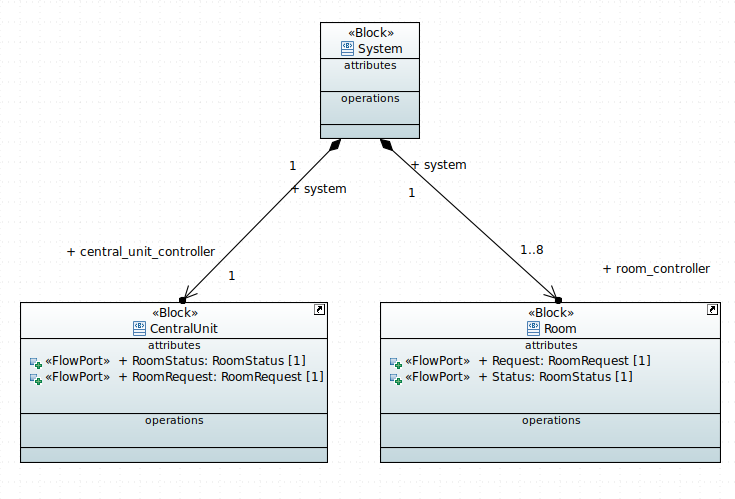
\includegraphics[width=12cm,keepaspectratio]{img/sysml/SystemComponents}
	\caption{System Components}
	\label{fig:SystemComponents}
\end{figure}
\begin{figure}[H]
	\centering
	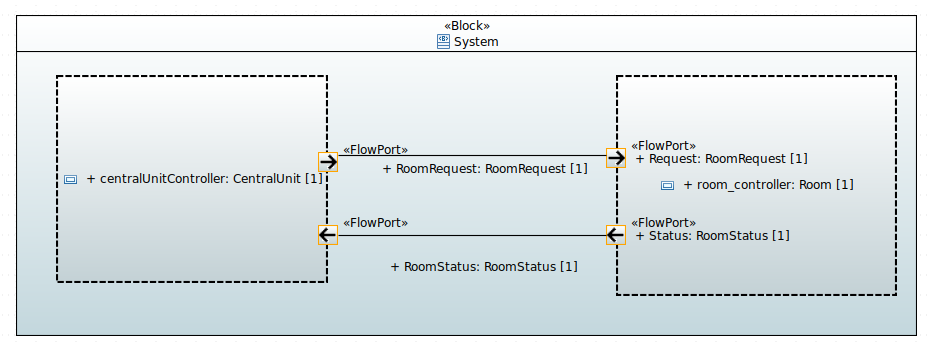
\includegraphics[width=12cm,keepaspectratio]{img/sysml/SystemInternals}
	\caption{System Internals}
	\label{fig:SystemInternals}
\end{figure}

\subsection{Central Unit}
The \textit{Central Unit} is composed by two modules, the \textit{RoomsManager} and the \textit{UserInterfaceManager}.
The \textit{RoomsManager} implements the functionalities related to the status of each room.
The \textit{UserInterfaceManager} that implements the functionalities related to represent the status of the system.
The two components exchange data as shown in \ref{fig:CentralUnit_internals}.
\begin{figure}[H]
	\centering
	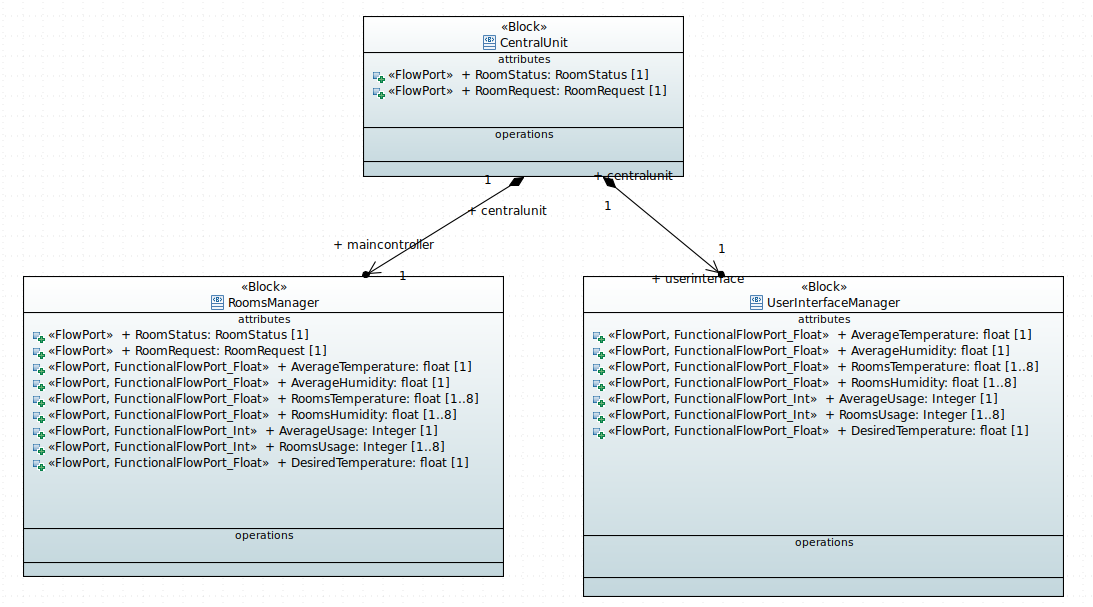
\includegraphics[width=12cm,keepaspectratio]{img/sysml/CentralUnitComponents}
	\caption{Central Unit components}
	\label{fig:CentralUnit_components}
\end{figure}

\begin{figure}[H]
	\centering
	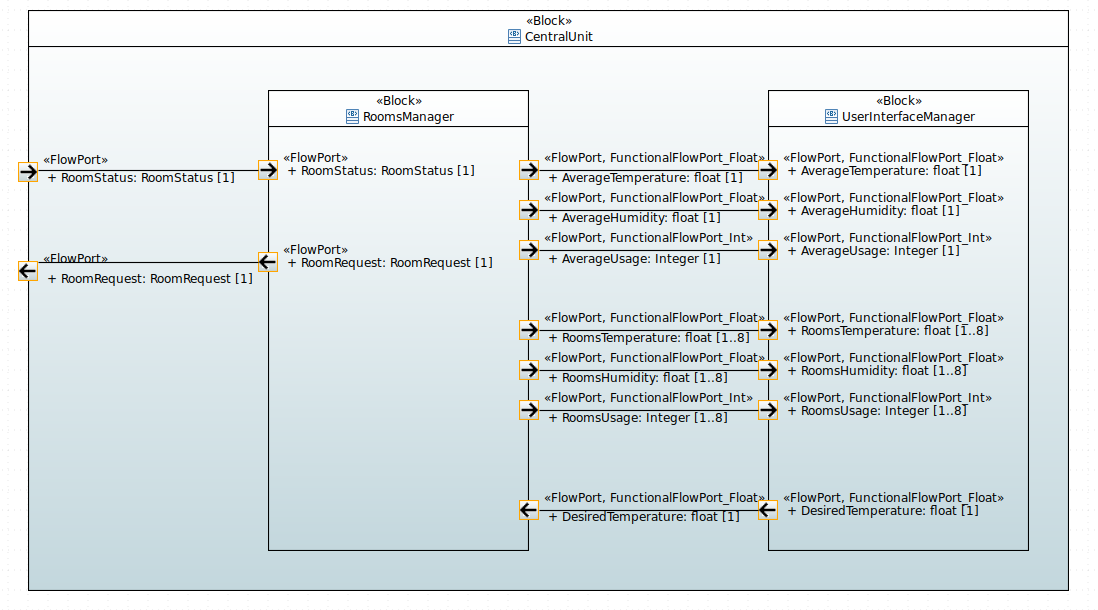
\includegraphics[width=12cm,keepaspectratio]{img/sysml/CentralUnitInternals}
	\caption{Central Unit internals}
	\label{fig:CentralUnit_internals}
\end{figure}

\subsection{Room module}
The main component of this module is the \textit{MainController} composed by different functions as shown in \ref{fig:RoomInternals}.
\begin{figure}[H]
	\centering
	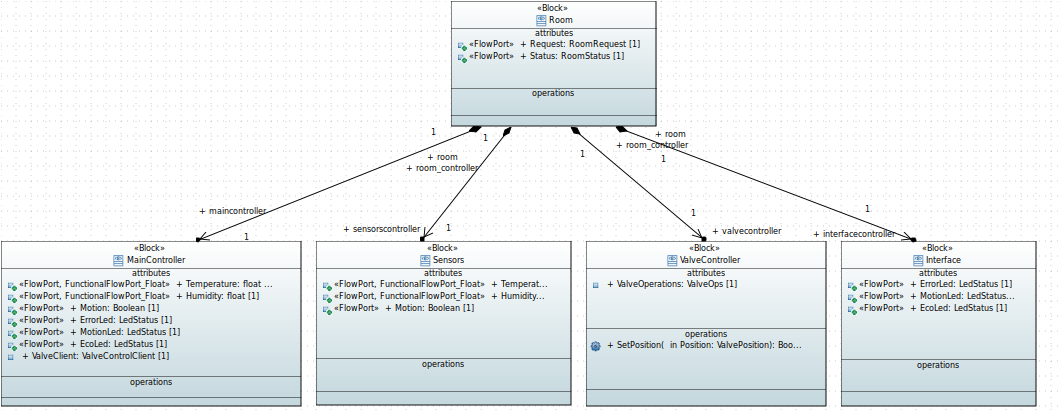
\includegraphics[width=13cm,keepaspectratio]{img/sysml/RoomComponents}
	\caption{Room Components}
	\label{fig:RoomComponents}
\end{figure}

\begin{figure}[H]
	\centering
	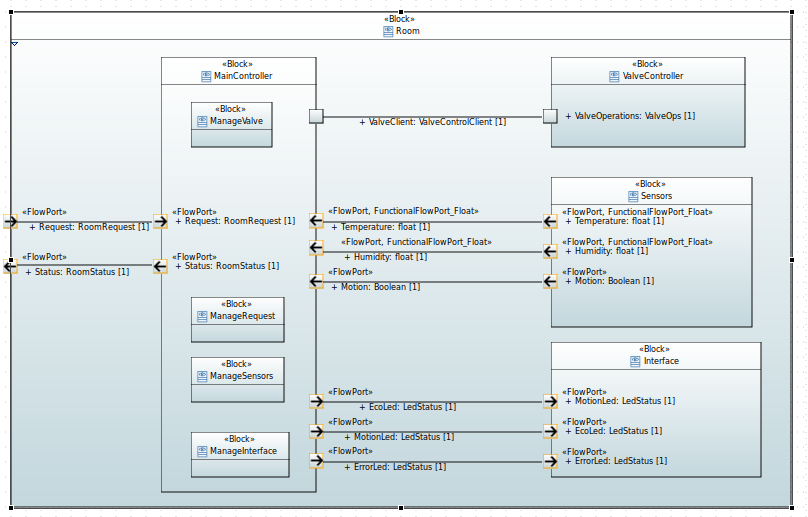
\includegraphics[width=13cm,keepaspectratio]{img/sysml/RoomInternals}
	\caption{Room Internals}
	\label{fig:RoomInternals}
\end{figure}

\begin{figure}[H]
	\centering
	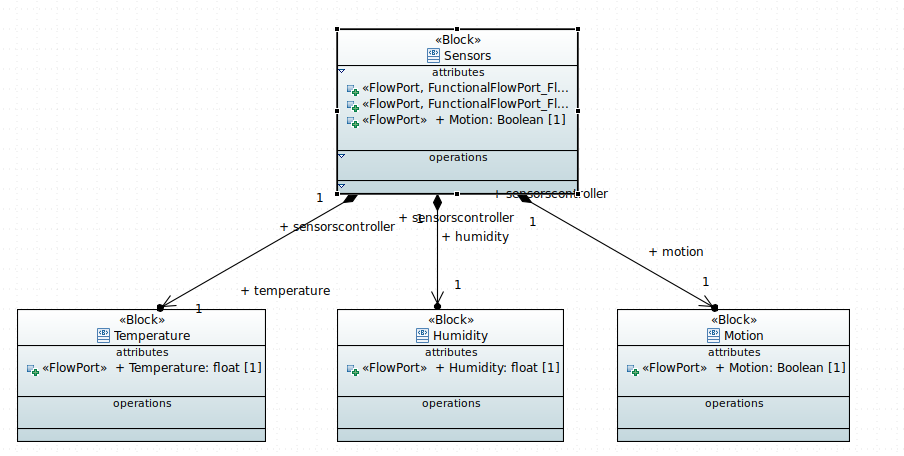
\includegraphics[width=13cm,keepaspectratio]{img/sysml/SensorsComponents}
	\caption{Room sensors components}
	\label{fig:room_sensors_components}
\end{figure}

\begin{figure}[H]
	\centering
	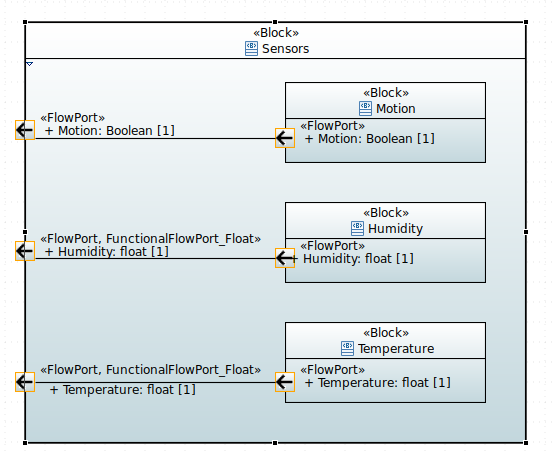
\includegraphics[width=8cm,keepaspectratio]{img/sysml/SensorsInternals}
	\caption{Room sensors internals}
	\label{fig:room_sensors_internals}
\end{figure}

\begin{figure}[H]
	\centering
	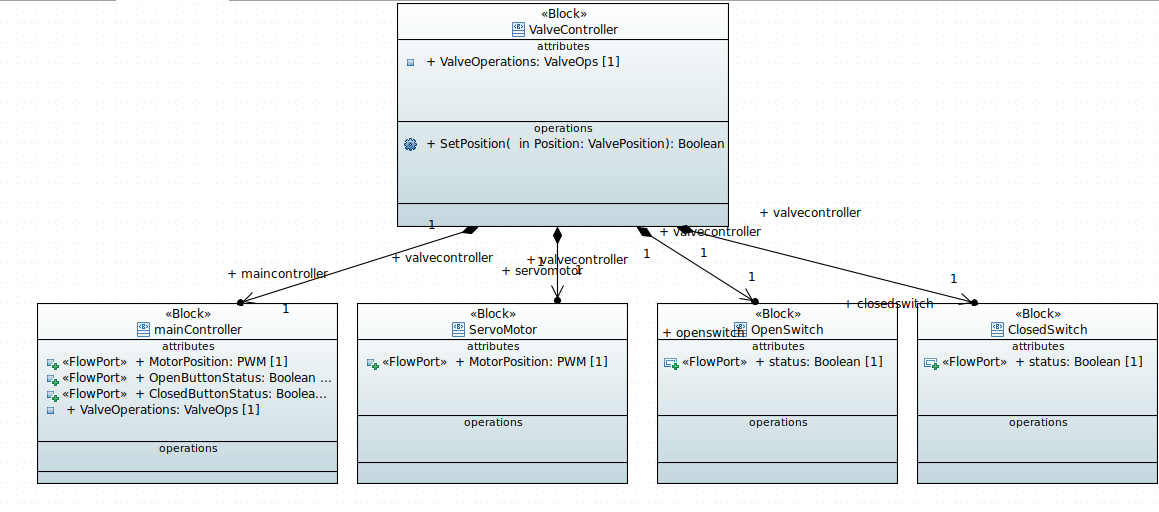
\includegraphics[width=12cm,keepaspectratio]{img/sysml/ValveControllerComponents}
	\caption{Valve Controller components}
	\label{fig:valve_dbd}
\end{figure}

\begin{figure}[H]
	\centering
	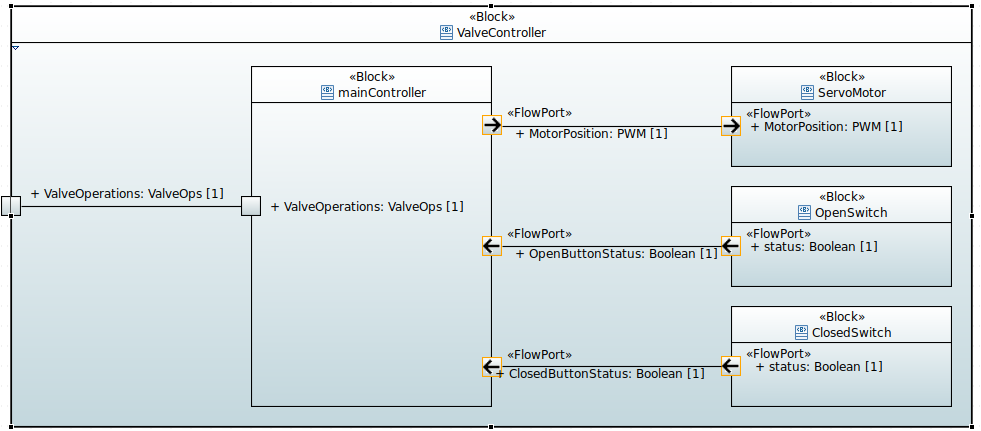
\includegraphics[width=12cm,keepaspectratio]{img/sysml/ValveControllerInternals}
	\caption{Valve Controller internals}
	\label{fig:valve_internals}
\end{figure}

\subsection{Communication State Machines}
In the following pictures are illustrated the behaviour of the communication between the \textit{CentralUnit} and the \textit{Room}.

\begin{figure}[H]
	\centering
	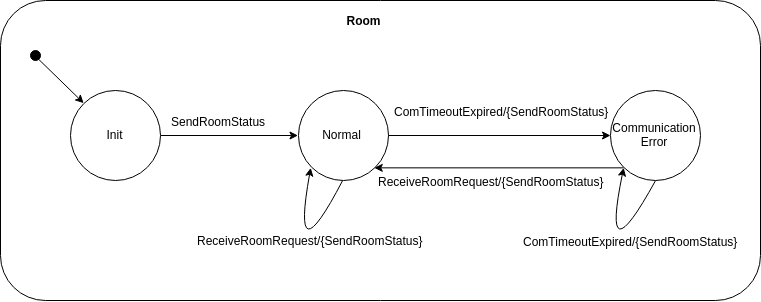
\includegraphics[width=12cm,keepaspectratio]{img/Com_SM_Room}
	\caption{Room communication management}
	\label{fig:room_com}
\end{figure}

In the figure \ref{fig:CU_com_receiver} is described the behaviour of the receiver part in the \textit{CentralUnit}, for readibility is reported just the case of a paramentric room X.\\

In the figure \ref{fig:CU_com_sender} is described the behaviour of the sender part in the \textit{CentralUnit}, for readibility is reported just the case of 2 rooms.

\begin{figure}[H]
	\centering
	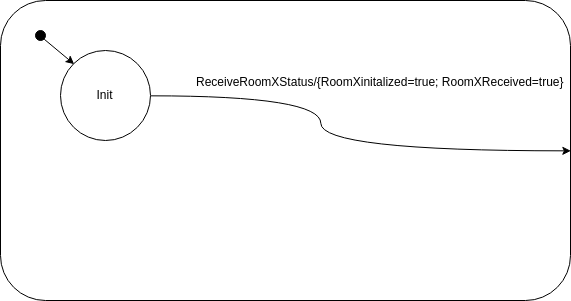
\includegraphics[width=10cm,keepaspectratio]{img/Com_SM_CU_Receiver}
	\caption{Central Unit communication receiver management}
	\label{fig:CU_com_receiver}
\end{figure}

\begin{figure}[H]
	\centering
	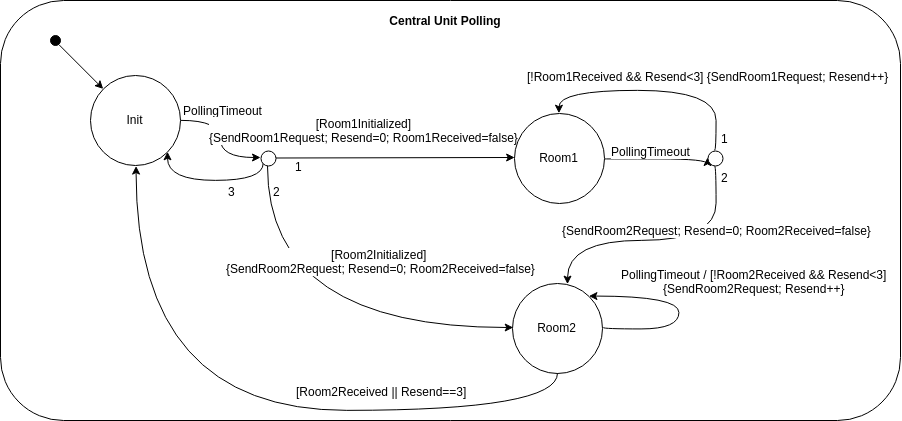
\includegraphics[width=12cm,keepaspectratio]{img/Com_SM_CU_Sender}
	\caption{Central Unit communication sender management}
	\label{fig:CU_com_sender}
\end{figure}


\end{document}